\documentclass[../main.tex]{subfiles}

\begin{document}
\section{Task 1 -- XGBoost}
The model was trained using mostly default parameters of the Python
\verb`xgboost` module. Despite this, it managed to achieve quite tremendous
results, as visible in table \ref{table:perf}.

\subsection{Model visualization}
\begin{figure}[H]
	\centering
	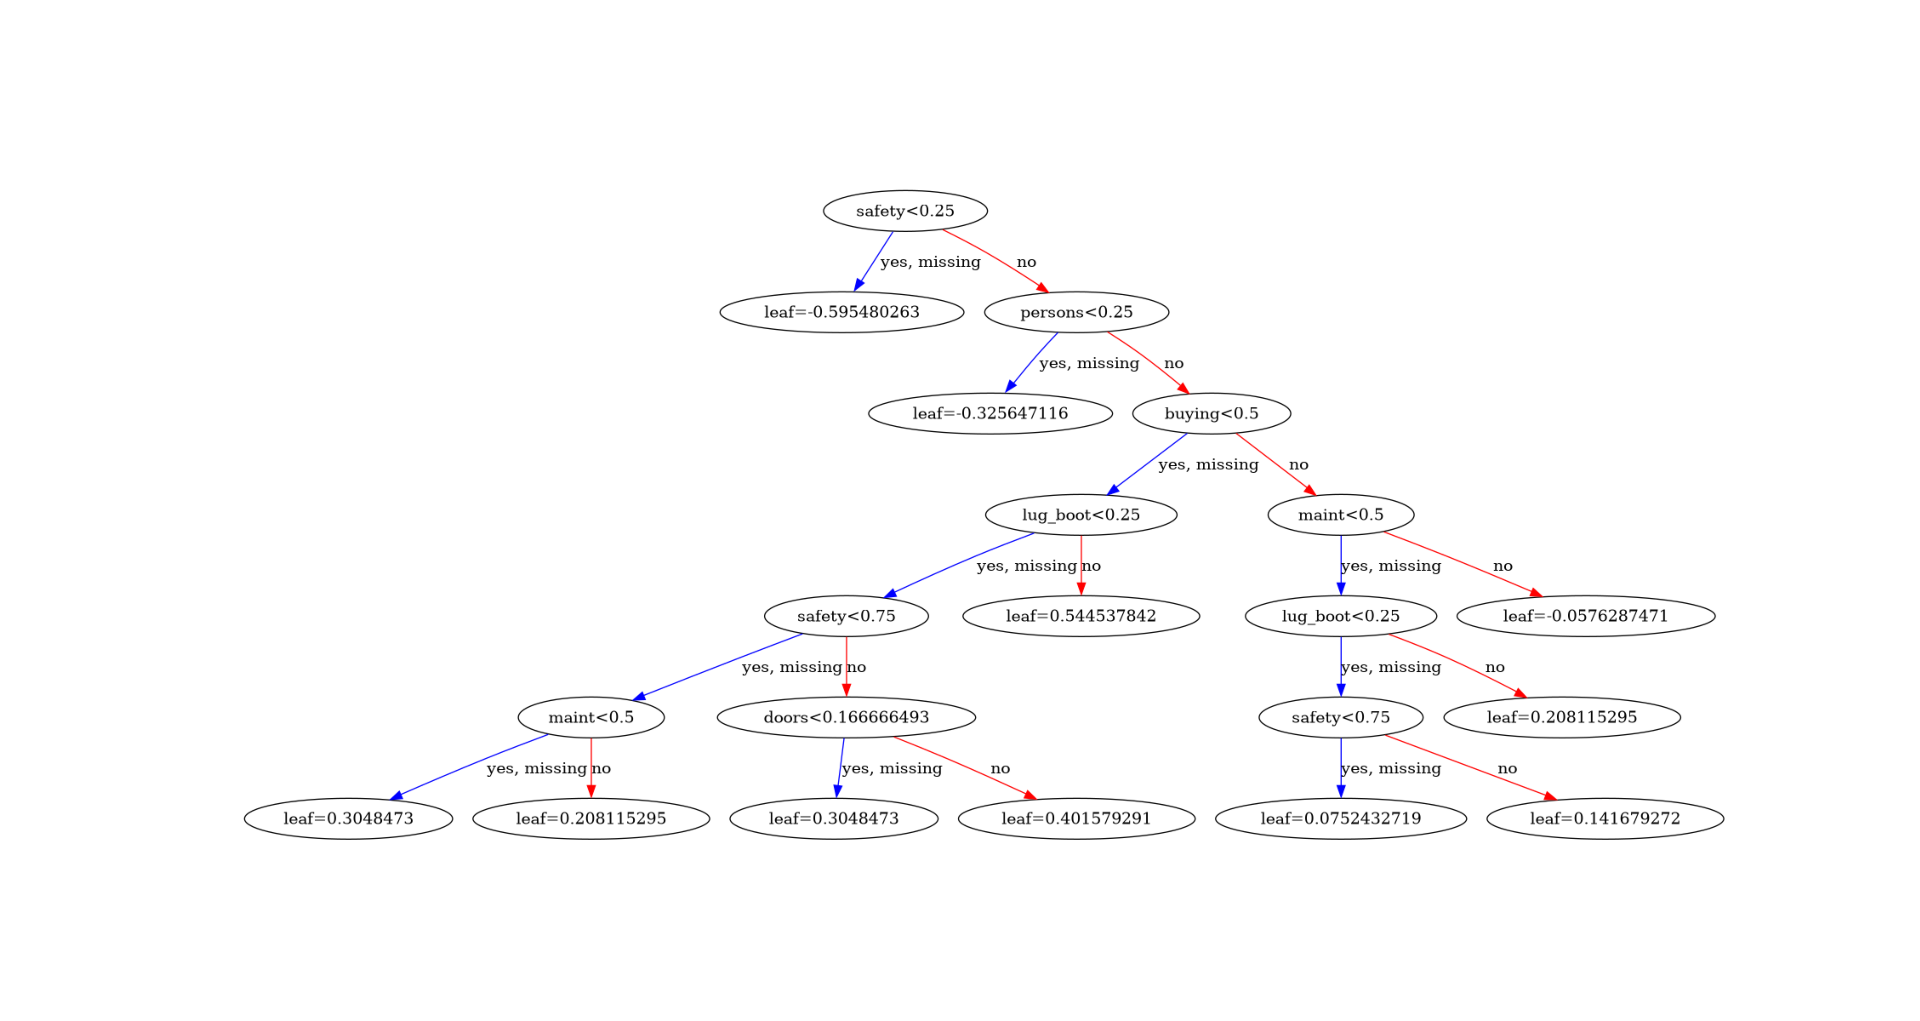
\includegraphics[width=\linewidth]{../img/xgb-tree.png}
	\caption{Last tree in the ensemble produced by XGBoost}
	\label{fig:xgb-tree}
\end{figure}

\subsection{Preference analysis}
\begin{figure}[H]
	\centering
	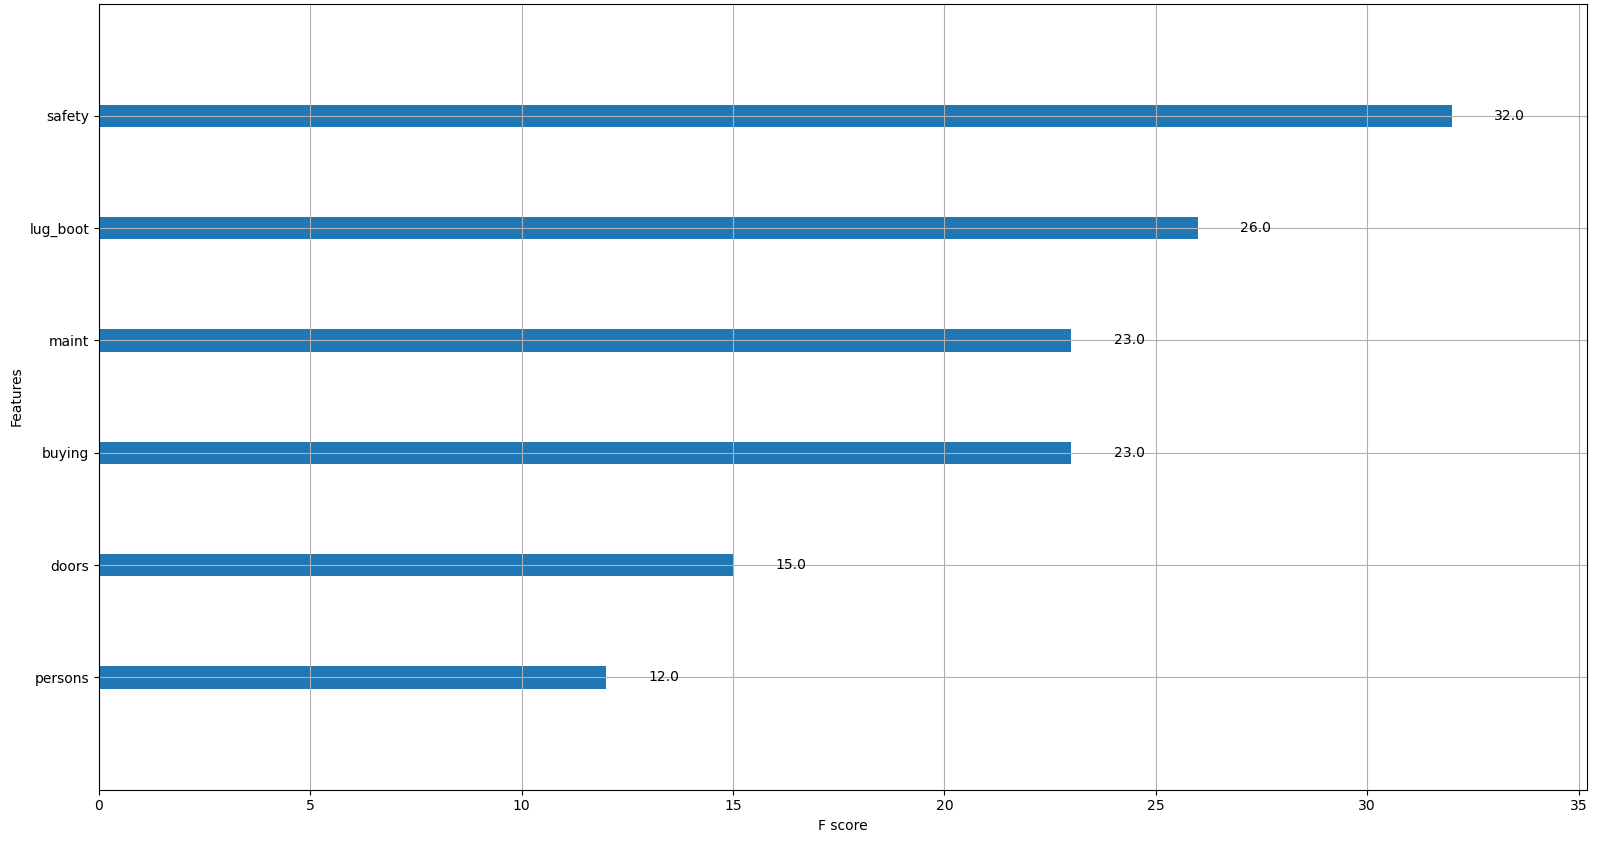
\includegraphics[width=\linewidth]{../img/xgb-feature-importance.png}
	\caption{XGBoost feature importance as computed by DALEX}
	\label{fig:xgb-feats}
\end{figure}
DALEX assigns very high importance to \emph{persons} and \emph{safety}, in that
order. This aligns with figure \ref{fig:xgb-3alt-allcetpar} of the forthcoming
ceteris paribus analysis. These importances don't fully agree with the above
model visualization (in which \emph{safety} seems to play a more significant
role), but it is important to keep in mind that the visualization is merely of
a single tree in an ensemble.

\paragraph{XGBoost} The XGBoost library also has native support for quantifying
and plotting feature importance. It must use a slightly different method than
DALEX, because the assigned values and even the ranking of the features are not
the same. For the sake of inter-model comparability, we prioritized the DALEX
output, but nevertheless this interpretation is also interesting:
\begin{figure}[H]
	\centering
	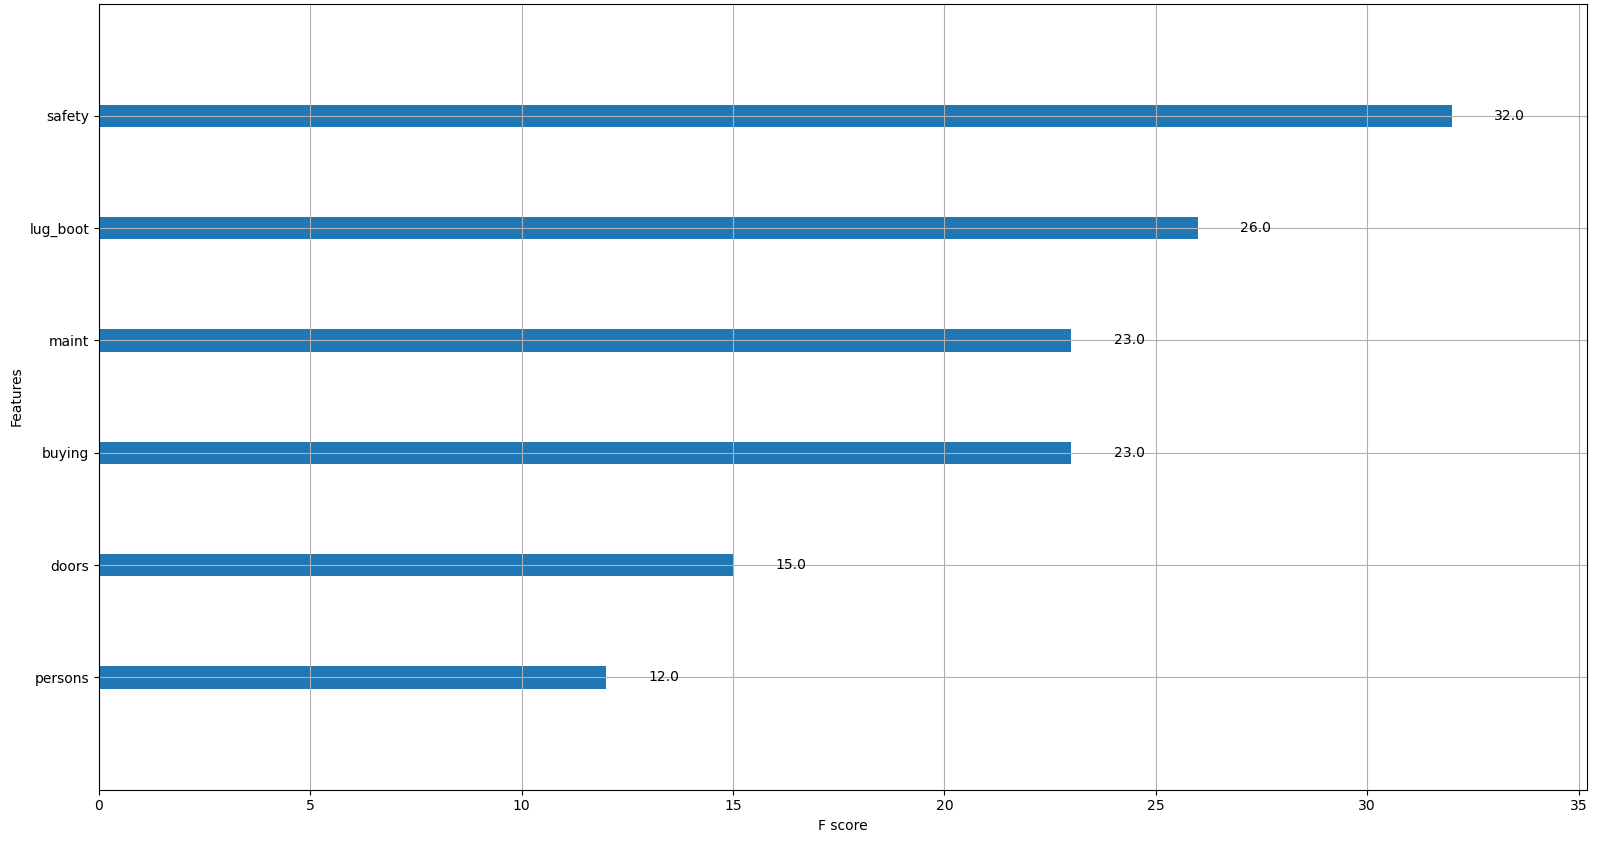
\includegraphics[width=\linewidth]{../img/xgb-feature-importance-xgboost.png}
	\caption{Importance of each feature, according to XGBoost}
	\label{fig:xgb-feats-xgboost}
\end{figure}
What is quite frankly shocking is the assignment of the lowest importance score
to \emph{persons}. This runs counter to both our intuitive expectations and
other analyses.

\subsection{3-alternative analysis}
\subsubsection{Analytical approach}
Predicting the outcome of a tree ensemble method is certainly not as trivial as
doing so with only a single tree. However, for the sake of simplicity, I will
assume that a single tree is a sufficiently accurate approximation of the
entire model and make judgements based on the final tree in the ensemble
produced by XGBoost, as seen on figure \ref{fig:xgb-tree}.
\paragraph{Alternative 1} This alternative has 0 \emph{safety}, which
disqualifies it on the very first tree branch (we want a positive leaf value).
Following the model's parameters, it would need a \emph{safety} of at least
0.25. Using the same logic for subsequent branches, \emph{persons} would
need to be at least 0.25 as well. From there the tree becomes more
complex, so I will assume a simple greedy strategy and only tweak feature
values when absolutely necessary. We proceed to the right with \emph{buying}
unchanged. Then we must lower \emph{maint} by more than 0.5. After
that, all leaves are positive, so there is no need for further changes.

\noindent
To sum up:
\begin{itemize}
	\item \emph{safety} 0.0 → 0.25
	\item \emph{persons} 0.0 → 0.25
	\item \emph{maint} 1.0 → 0.49
\end{itemize}

\paragraph{Alternative 2} Using the same procedure as with alternative 1, we
get:
\begin{itemize}
	\item \emph{safety} 0.0 → 0.25
\end{itemize}
\paragraph{Alternative 3} Same procedure once more, but this time we are aiming
for the unacceptable class:
\begin{itemize}
	\item \emph{safety} 1.0 → 0.24
\end{itemize}

\subsubsection{Space sampling}
To concisely show how changing the value of just one attribute would change the
result, ceteris paribus analysis was performed.

Most plots were approximately "flat", with no major shifts in prediction
(Y-axis). What this generally means is that those features alone can't swivel
the classification of an alternative.

There are, however, 2 features that do exhibit some major shifts --
\emph{safety} and \emph{persons}. Files with all plots are available in
\verb`report/img/extras`. In order not to overcrowd the report, only the plots
for \emph{safety} and \emph{persons} for the 3 alternatives are presented.

\begin{figure}[H]
	\centering
	\begin{subfigure}[b]{0.32\linewidth}
		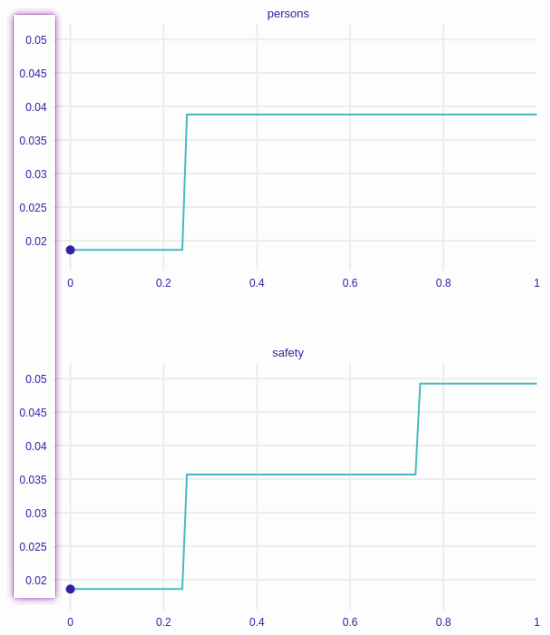
\includegraphics[width=\linewidth]{../img/xgb-cetpar-worst.png}
		\caption{alternative 1 (worst)}
		\label{fig:xgb-3alt1-cetpar}
	\end{subfigure}
	\begin{subfigure}[b]{0.32\linewidth}
		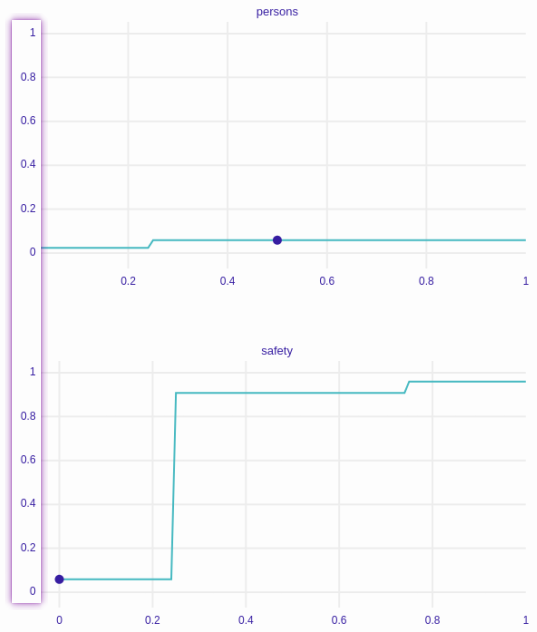
\includegraphics[width=\linewidth]{../img/xgb-cetpar-mid.png}
		\caption{alternative 2 (mid)}
		\label{fig:xgb-3alt1-cetpar}
	\end{subfigure}
	\begin{subfigure}[b]{0.32\linewidth}
		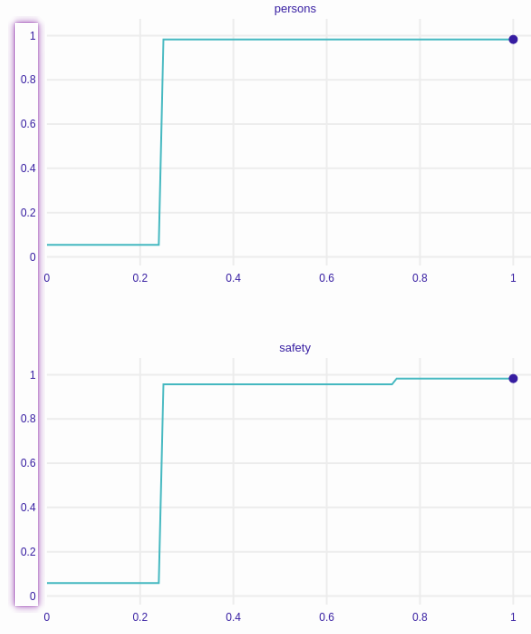
\includegraphics[width=\linewidth]{../img/xgb-cetpar-best.png}
		\caption{alternative 3 (best)}
		\label{fig:xgb-3alt1-cetpar}
	\end{subfigure}
	\caption{Ceteris paribus of \emph{persons} and \emph{safety} features in XGBoost}
	\label{fig:xgb-3alt-allcetpar}
\end{figure}
For alternative 2, \emph{safety} is very highly correlated with the decision
class. There is a clear boundary at around 0.25 where the model leaps from
being barely above 0 to being almost 1. This suggests that there were many
middle alternatives which were unacceptable solely due to a low \emph{safety}
value. The same observation can be made for alternative 3 (both
\emph{persons} and \emph{safety}).

A bonus observation is that these plots resemble \textbf{step functions}. That
is because XGBoost is a tree ensemble model, and trees are unable to produce
smooth decision boundaries due to their nature of branching on specific feature
values.

\paragraph{Alternative 1} Applying the changes suggested in the
\emph{Analytical approach} section did not produce the wanted change, but it
did increase the overall score from \verb`0.02` to \verb`0.38` (on a range from
\verb`0.0` to \verb`1.0` and a binary decision boundary \verb`0.5`).
\paragraph{Alternative 2} Increasing \emph{safety} to 0.25 yielded a change
from \verb`0.06` to a whopping \verb`0.91`. This further reinforces the idea
that \emph{safety} plays a dominant role in predicting the outcome class.
\paragraph{Alternative 3} Decreasing \emph{safety} to 0.24 reduced the score
from \verb`0.98` to \verb`0.06`. Once again, \emph{safety} proves critical.

\subsubsection{Variable contribution plots}
\begin{figure}[H]
	\centering
	\begin{subfigure}{\linewidth}
		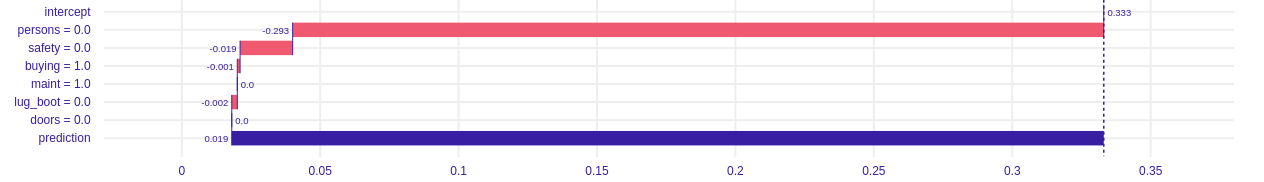
\includegraphics[width=\linewidth]{../img/xgb-breakdown-worst.png}
		\caption{alternative 1 (worst)}
		\label{fig:xgb-3alt1-contrib}
	\end{subfigure}
	\begin{subfigure}{\linewidth}
		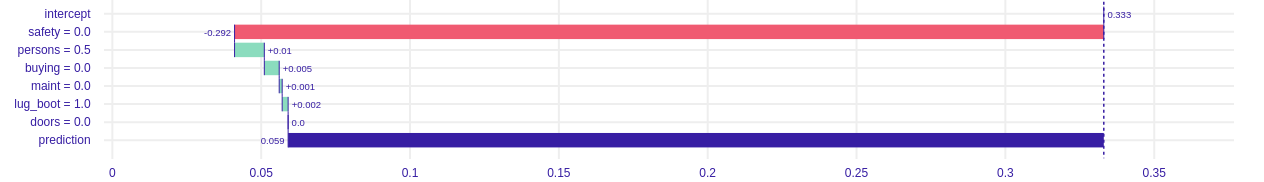
\includegraphics[width=\linewidth]{../img/xgb-breakdown-mid.png}
		\caption{alternative 2 (mid)}
		\label{fig:xgb-3alt2-contrib}
	\end{subfigure}
	\begin{subfigure}{\linewidth}
		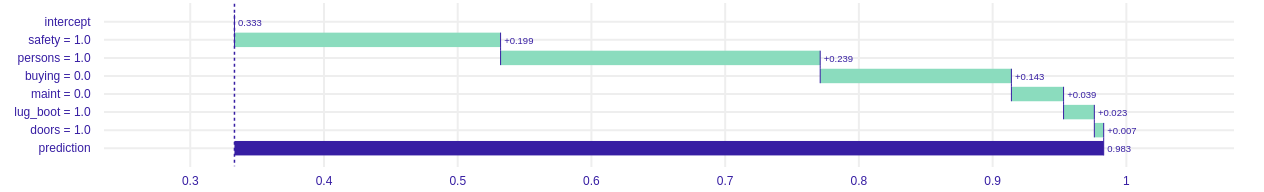
\includegraphics[width=\linewidth]{../img/xgb-breakdown-best.png}
		\caption{alternative 3 (best)}
		\label{fig:xgb-3alt3-contrib}
	\end{subfigure}
	\caption{Variable contributions of 3 alternatives in XGBoost}
	\label{fig:xg-3alt-allcontrib}
\end{figure}
The variable contribution plots reveal a striking imbalance between the
features in the XGBoost model. For low and mid ranking alternatives, almost all
of the negative feedback is attributed to \emph{safety} or \emph{persons}, with
remaining features hardly affecting the overall prediction score.

The high ranking alternative is much more uniform, with \emph{doors} having the
smallest contribution.
\end{document}
